%\section{Features} \label{sec:features}
% Dr Denes: can keep, but removed for now to condense
%Rich data is valuable, however, irrelevant or redundant variables can increase both training and inference time, as well as decrease a model's performance, therefore choosing appropriate features to input into a classification model is very important.

\subsection{Match Representation}
We represent each match from a participating player's perspective as follows:
%In supervised machine learning, a set of labelled data is required for the model to train on. In the context of table tennis prediction, each match corresponded to two instances of data, one from the perspective of each player respectively, where every sample is composed of two elements:
\begin{itemize}
    \item a feature vector ($\underline{x}$) consisting of player and previous match statistics,
    \item{
     the target variable ($y$), indicating the result of the match: %that corresponds to its respective sample
     \begin{equation}
        y =
        \begin{cases}
        1, &\text{if $player_i$ wins} \\ 
        -1, &\text{if $player_i$ loses}
        \end{cases}.
    \end{equation}
     }
\end{itemize}



With incomplete matches removed from the dataset, there are no other possible outcomes (i.e. no draws in table tennis). Each match maps to two ($\underline{x}$,$y$) pairs, from the perspective of the two participating players.
%As any incomplete matches were removed from the dataset, 

\subsection{Feature Engineering}
\label{sec:engineer}
We followed the approaches taken in \textit{tennis}  \cite{barnett2005combining,sipko2015machine,cornman2017machine}  to form new features for table tennis. These features are player-focused, as unlike in team sports, we do not need to consider line-ups, collective team ability or substitutions.

%Using pre-existing knowledge on the sport, adding combinations of player statistics as features may improve the predictive model. These features were calculated as differences between different player statistics as this considers the characteristics of \textit{both} players participating in a match. This was inspired by 

%In table tennis, there are only two possible outcomes of a match; a win or a loss. 


Table~\ref{table:nonlin} shows the final  set of features. Newly derived features are indicated with *. More detailed explanations can be found in subsections below.
%\ref{sec:sp} to \ref{sec:balance}.

\begin{table}[ht]
\caption{Feature Summary} % title of Table
\centering % used for centering table
\setlength{\tabcolsep}{3pt}
\scalebox{1.2}{%
\begin{tabular}{c c} % centered columns (4 columns)
\hline\hline %inserts double horizontal lines
Feature & Explanation \\ [0.5ex] % inserts table

%heading
\hline % inserts single horizontal line
SP & percentage of total points won on serve \\
RP & percentage of total points won on receive \\
LRP & percentage of total points won on a long rally \\
SRP & percentage of total points won on a short rally \\
FHP & percentage of total points won on a forehand \\
BHP & percentage of total points won on a backhand \\ 
RANK & player ranking \\
RANKDIFF* & difference in rank between opponents \\
SA* & player serve advantage \\
SRA* & player short rally advantage \\
FHA* & player forehand advantage \\
BALANCE* & measure of how well rounded a player is \\
[1ex] % [1ex] adds vertical space

\hline %inserts single line
\end{tabular}}
%\vspace{4em}

\label{table:nonlin} % is used to refer this table in the text
\end{table}


\subsubsection*{SP: Serve Percentage}\label{sec:sp}
The proportion of points won on serve by a player. 
%This can be demonstrated from data similar to \figref{sequence}; 
If the serve and error are made on opposing sides of the table, it  was won by the serving player.

\subsubsection*{RP: Receive Percentage}\label{sec:rp}
The proportion of points won by the receiving player. E.g. in \figref{sequence}, the serve and error is made by the same player, so the point is won by the receiver.

\subsubsection*{LRP: Long Rally Percentage}\label{sec:lrp}
%\denes{ I'm confused again about the meaning of a long vs short rally}.
The proportion of points won on a long rally by a player to the total number of rallies won. In this paper we define a long rally as a rally of at least five shots. E.g. \figref{svlr} shows that one player won 47 points on a long rally, while the other won 45.
%\denes{how do we get percentage?}.

\subsubsection*{SRP: Short Rally Percentage}\label{sec:srp}
Compared to LRP, this is the proportion of points won on a \textit{short rally} by a player. E.g. \figref{svlr} shows that one player won 21 points on a short rally, while the other won 24 in the entire match.

\subsubsection*{FHP: Forehand Percentage}\label{sec:fp}
The proportion of points won on a forehand by a player, determined by the type of stroke used on the winning shot of a rally. \figref{fvbh} shows one player won 24 points on a forehand, and the other winning 38.

\subsubsection*{BHP: Backhand Percentage}\label{sec:bp}
The proportion of points won on a backhand by a player. \figref{fvbh} shows one player won 43 points on a backhand, and the other winning 29.

\subsubsection*{RANK} \label{sec:rank}
The ranking of the player by ITTF 
%\denes{who establishes the ranking? ITTF?}

\subsubsection*{RANKDIFF*: Rank Difference} \label{sec:rankdiff}
Constructed by calculating the difference between rankings of two opponents:
\begin{equation}
    \text{RANKDIFF} = \begin{cases}
\text{RANK}_i - \text{RANK}_j &\text{for player $i$} \\
\text{RANK}_j - \text{RANK}_i &\text{for player $j$},
\end{cases}
\end{equation}
where RANK$_i$ and RANK$_j$ are respective player rankings at the time of the match. A rank advantage (i.e. lower numerical value than an opponent's), yields a negative RANKDIFF. Rankings are mostly reliable for the top players; for example, players of rank 2 and rank 7 is much more likely to have an accurate depiction of their standard in comparison to two players of rank 150 and 155, despite the rank difference being the same. To account for this, we apply a simple non-linearity and set RANKDIFF to $0$ for matches where both players are ranked above 100.%, the feature  is ignored ($=0$). This is due to the fact that the lower the rank of a player, the more likely it is that there will be other players of a similar standard where rank doesn't accurately represent the standard of a player.


\subsubsection*{SA*, SRA*, HA*} \label{sec:advantage}
The serve advantage of a player is calculated as the difference between their serve and receive winning percentage. This depicts the contrast as to how likely a player is to win a point if they are serving rather than if they are on receive. Subsequently, the advantage a respective player has in a short rally over a long rally, as well as the advantage a respective player has in a forehand stroke over a backhand stroke, can be calculated therefrom.

\subsubsection*{BALANCE*} \label{sec:balance}

Players of a higher skill level tend to have fewer weaknesses and are stronger in more aspects of the game. We propose measuring the overall well-roundness of a player as:
\begin{equation}
    \textit{BALANCE} = \frac{|\textit{SA}|+|\textit{SRA}|+|\textit{FHA}|}{3}.
\end{equation}

\denes{please see if we can refit the model with player profiles based on aggregate match data; or alternatively plot these features as they progress through time so we can argue that this still allows us to do during-match prediction}
\sophie{I've plotted how different features vary over time, they seem to converge probably around the second to third set. Thoughts? I've also averaged out all features from past matches for each player and used those values for prediction on the test set for pre-match prediction.
This also means pre-match predictions can't be made for new players.}

\begin{figure}[ht]
\centering

%\vspace{-2em}
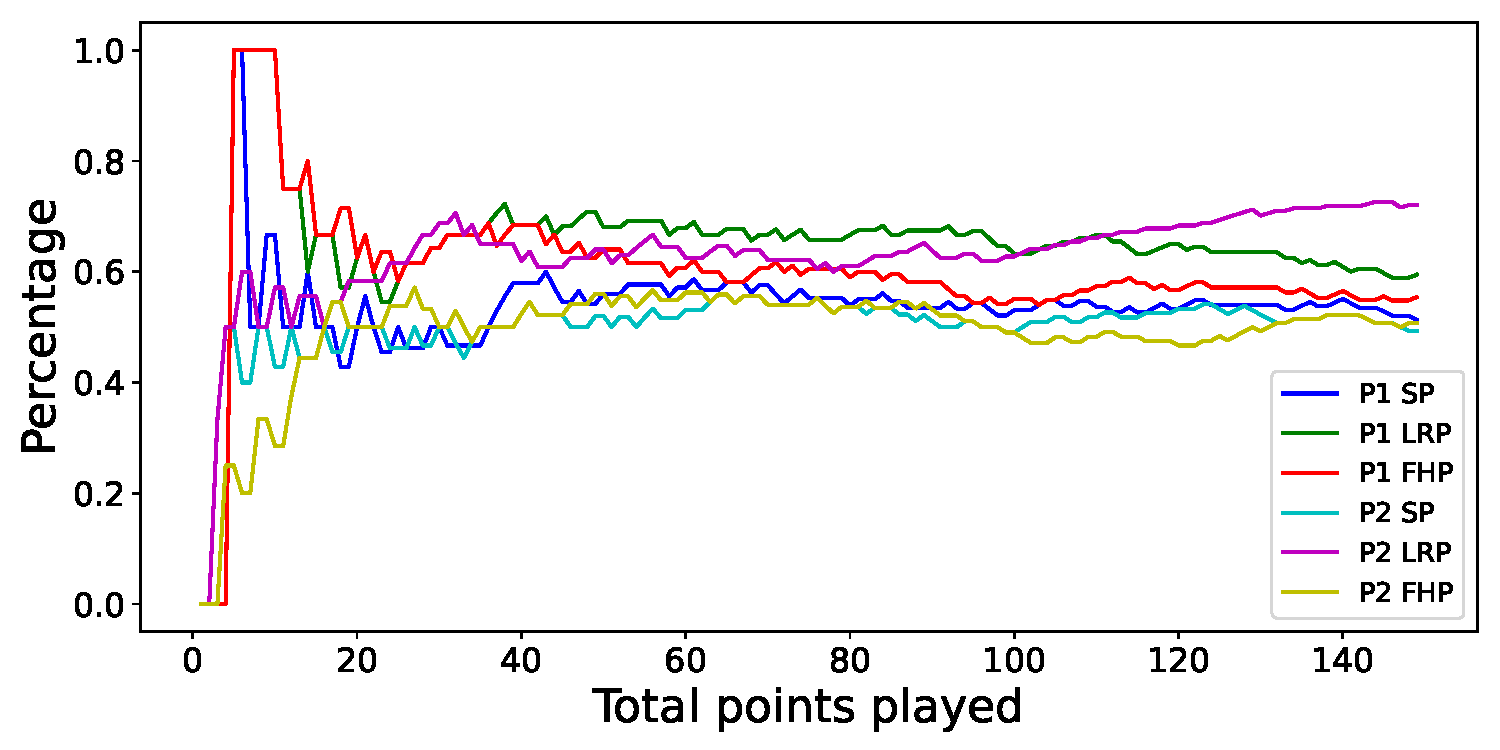
\includegraphics[width=8cm]{plots/featuresandtime.pdf}
\caption{Features plotted against the course of the match for both players.}

\label{fig:time}
\end{figure}

\begin{table}[ht]
\caption{Pre-match prediction model performance}
\label{prematch}
\centering
\setlength{\tabcolsep}{10pt}
\scalebox{1.05}{%
\begin{tabular}{ l|c c }

\multirow{2}{4em}{Model} &
\multicolumn{2}{|c}{Test set} \\
\cline{2-3} & Acc & F1 \\

\hline \hline 
Logistic Regression & 0.639 & 0.667 \\
Random Forest & 0.667 & 0.714 \\
Support Vector Machine & & \\
$\rightarrow$ Linear & 0.639 & 0.667 \\
$\rightarrow$ RBF    & 0.639 & 0.649 \\
$\rightarrow$ Polynomial & 0.611 & 0.632\\
$\rightarrow$ Sigmoid & 0.639 & 0.649 \\
MLP Neural Network & 0.667 & 0.714\\
[1ex]
\hline
\end{tabular}}
\end{table}

\subsection{Feature Scaling}
To account for the varying numerical range of the input features, and to make features comparable, we standardise each input to a zero mean with a unit standard deviation.
%Different features tend to have a varying range of values, therefore it is best practice to scale features as part of data pre-processing prior to learning. \textit{Standardization} is a scaling technique to centre values around the mean with a unit standard deviation \cite{bollegala2017dynamic}. We get a coded value by subtracting the mean of the sample from the data and dividing it by the standard deviation. The feature representing rank difference for example, is represented across a much larger range compared to features which are percentages.
